% !TEX encoding = UTF-8
\documentclass[UTF8]{ctexart}

\usepackage[utf8]{inputenc}
\usepackage{graphicx}
\usepackage{geometry}
\geometry{a4paper}
\geometry{left=2.5cm,right=2.5cm,top=2.8cm,bottom=1.3cm}

\usepackage{booktabs}
\usepackage{array}
\usepackage{paralist}
\usepackage{verbatim}
\usepackage{subfig}
\usepackage{amsmath}
\usepackage{mathtools}
\usepackage{listings}
\usepackage[table]{xcolor}
\usepackage{lastpage}
\usepackage{url}

% Using hyperref for improved ref character
\usepackage[colorlinks,linkcolor=black,anchorcolor=black,
citecolor=black,CJKbookmarks=True]{hyperref}

% For picture drawing
\usepackage[all]{xy}

% For code inserting. Set features.
\lstset{
alsolanguage=matlab,
tabsize=4,
keepspaces=true,
numbers=left,
numberstyle=\tiny,
keywordstyle=\color{blue!70} \bfseries,
commentstyle=\color{red!50!green!50!blue!50},
frame=shadowbox,
breaklines,
showspaces=false,
showstringspaces=false,
showtabs=false,
rulesepcolor=\color{red!20!green!20!blue!20},
extendedchars=false,
escapeinside=``
}

% Set the font of page header
\usepackage{fancyhdr}
\pagestyle{fancy}
\lhead{传感器特性实验报告}
\chead{}
\rhead{Page \thepage/\pageref{LastPage}}
\cfoot{}
\rfoot{}
\lfoot{}

\usepackage{sectsty}

\usepackage[nottoc]{tocbibind}
\usepackage[titles,subfigure]{tocloft}
\renewcommand{\cftsecfont}{\rmfamily\mdseries\upshape}
\renewcommand{\cftsecpagefont}{\rmfamily\mdseries\upshape}

% Set number of ref to be relevent to section number
\renewcommand{\theequation}{\arabic{section}.\arabic{equation}}
\renewcommand{\thefigure}{\arabic{section}-\arabic{figure}}
\renewcommand{\thetable}{\arabic{section}-\arabic{table}}
\makeatletter
\@addtoreset{equation}{section}
\@addtoreset{figure}{section}
\@addtoreset{table}{section}
\makeatother

% Set the font of the reference
\bibliographystyle{unsrt}

% Define user\rq{}s color
\usepackage{colortbl}
\definecolor{lightgray}{gray}{.9}
\definecolor{thickgray}{gray}{.6}

\usepackage{multirow}

% 首行缩进
\usepackage{indentfirst}

% Set section numbering
\CTEXsetup[number={}]{part}
\renewcommand{\thepart}{}
\usepackage{titlesec}
\titleformat{\part}[block]{\color{blue}\huge\bfseries\filcenter}{}{1em}{}

%\usepackage{ulem}
%\usepackage{indentfirst}
%\setlength\textwidth{300.0pt}
%

% 重定义字体命令
\newcommand{\song}{\CJKfamily{song}}    % 宋体   (Windows自带simsun.ttf)
\newcommand{\fs}{\CJKfamily{fs}}        % 仿宋体 (华天字库htfs.ttf)
\newcommand{\kai}{\CJKfamily{kai}}      % 楷体   (华天字库htkai.ttf)
\newcommand{\hei}{\CJKfamily{hei}}      % 黑体   (Windows自带simhei.ttf)
\newcommand{\li}{\CJKfamily{li}}        % 隶书   (Windows自带simli.ttf)
\newcommand{\you}{\CJKfamily{you}}      % 幼圆体 (Windows自带simyou.ttf)
%%%  以上六种字体均为标准 GBK 字体, 包括 GBK 繁体字和一些不常用字, 推荐!!!

\newcommand{\xs}{\CJKfamily{xs}}
\newcommand{\shu}{\CJKfamily{shu}}      % 舒体   (方正字库fzstk.ttf)
%  \newcommand{\yourcommand}[参数个数]{内容}   [参数个数]这个是可选的。
%  例如  \newcommand{\you}{\CJKfamily{you}}  用\you 来代替 \CJKfamily{you} ,少输入很多字哦。
%字号设置
\newcommand{\chuhao}{\fontsize{42pt}{\baselineskip}\selectfont}
\newcommand{\xiaochuhao}{\fontsize{36pt}{\baselineskip}\selectfont}
\newcommand{\yihao}{\fontsize{28pt}{\baselineskip}\selectfont}
\newcommand{\xiaoyihao}{\fontsize{24pt}{\baselineskip}\selectfont}
\newcommand{\erhao}{\fontsize{21pt}{\baselineskip}\selectfont}
\newcommand{\xiaoerhao}{\fontsize{18pt}{\baselineskip}\selectfont}
\newcommand{\sanhao}{\fontsize{15.75pt}{\baselineskip}\selectfont}
\newcommand{\sihao}{\fontsize{14pt}{\baselineskip}\selectfont}
\newcommand{\xiaosihao}{\fontsize{12pt}{\baselineskip}\selectfont}
\newcommand{\wuhao}{\fontsize{10.5pt}{\baselineskip}\selectfont}
\newcommand{\xiaowuhao}{\fontsize{9pt}{\baselineskip}\selectfont}
\newcommand{\liuhao}{\fontsize{7.875pt}{\baselineskip}\selectfont}
\newcommand{\qihao}{\fontsize{5.25pt}{\baselineskip}\selectfont}
% \baselineskip | distance from bottom of one line of a paragraph to bottom of the next line.  基本行距
%  只有使用\selectfont命令之后,\fontzize{}{}的设置才能生效
%  可以用数字表示{11pt}:单倍行距

\begin{document}
%%%%%%%%%%%%%%%%%%%%%%%%%%%%封面与目录%%%%%%%%%%%%%%%%%%%%%%%%%%%%%%
\begin{titlepage}
\begin{center}
% Upper part of the page

\includegraphics[width=0.25\textwidth]{resource/logo.jpg}\\[1cm]
\textsc{\LARGE Department of Automation}\\[1.5cm]
\fs{\Large 模式识别基础第二次作业}\\[0.5cm]
% Title
\hrulefill
\\[0.8cm]{\centering \huge \hei 用身高体重数据进行性别分类的实验(二)}\\[0.4cm]
\hrulefill
\\[4cm]

% Author and supervisor
\begin{tabbing}       %tabbing  列表

 \hspace*{5cm} \= \hspace{2.6cm} \= \kill
 % \=     in tabbing environment, sets a tab stop
 % \kill  in a\tabbing environment, deletes previous line so tabs can be set without outputting text.
 % \>     in tabbing environment is a forward tab.

\>{\fs\sihao\textbf {班\hspace{1cm}级 \ \ :}}\>  {\centering\fs\sihao\textbf{~~~~~~~~~自~~3~2}} \\
\\
\>{\fs\sihao\textbf {姓\hspace{1cm}名 \ \ :}}\>  {\centering\fs\sihao\textbf{~~~~~~~~陈~昊~楠}}\\
\\
\>{\fs\sihao\textbf {学\hspace{1cm}号 \ \ :}}\>  {\centering\fs\sihao\textbf{~~~~~~2013011449}}\\
\\
\>{\fs\sihao\textbf {授课教师 \ \ :}}\>  {\centering\fs\sihao\textbf{~~~~~~~~张~学~工}} \\

\end{tabbing}
\vfill
{\large \today}
\end{center}
\end{titlepage}

\tableofcontents
\clearpage

%%%%%%%%%%%%%%%%%%%%%%%%%%正文部分%%%%%%%%%%%%%%%%%%%%%%%%%%%%%%%%%%

\section{实验内容}
\begin{enumerate}
	\item 用 {\ttfamily dataset3} 作为训练数据,用 {\ttfamily dataset4} 作为测试数据,采用不同的特征、训练样本数、分类方法进行比较实验,观察、分析实验结果的异同。
	\begin{itemize}
		\item 特征组合
		\begin{enumerate}
			\item 10个特征都用
			\item 只用第3、5列特征
		\end{enumerate}
		\item 训练样本组合
		\begin{enumerate}
			\item 从dataset3 中任选20 个训练样本(男女各10 例)
			\item dataset3 中的全部训练样本
		\end{enumerate}
		\item 分类器方法
		\begin{enumerate}
			\item 最小错误率贝叶斯分类器(假设正态分布,先验概率各50\%)
			\item Fisher 线性判别(FLD)
			\item 线性SVM
			\item 采用BP 算法的MLP 神经网络(网络结构自定)
		\end{enumerate}
	\end{itemize}
	\item 汇总测试错误率
	\item 结合实验观察和对各种方法特点的理解,尝试对训练样本数、特征维数以及所选用的方法与测试结果的关系进行讨论。
	\item (选做)选择具有代表性的实验结果,设法在由第3 列和第5 列特征组成的平面上粗略画出不同样本数和特征数下得到的分类器,观察分析所得分类器特性与样本数、特征、分类方法之间的关系。
\end{enumerate}

\section{实验方法}
\subsection{Bayes最小错误率分类}
该方法假设男性、女性两类之内对所有特征服从多维正态分布。设两类的均值、协方差矩阵分别为$\mu_i,\Sigma_i\quad i=1,2$,则决策边界可按式\ref{eq:bayes}计算:
\begin{equation}
\label{eq:bayes}
-\frac12[(x-\mu_i)^\mathbf{T}\Sigma_i^{-1}(x-\mu_i)-(x-\mu_j)^\mathbf{T}\Sigma_j^{-1}(x-\mu_j)]-\frac12\ln \frac{|\Sigma_i|}{|\Sigma_j|}+\ln\frac{P(\omega_i)}{P(\omega_j)}=0
\end{equation}
若假设先验概率均为$0.5$,则上式最后一项可以忽略。
\subsection{Fisher线性分类器}
二分类的线性判别函数的一般表达式为
\begin{equation}
f(\mathbf{x}) = \mathbf{w}^T \mathbf{x} + b
\end{equation}
该方法可以看作将所有样本投影到一维,并根据阈值$b$进行分类。Fisher线性判别的思想就是,选择投影方向,使得投影后两类相隔尽可能远,而同时每一类内部的样本又尽可能聚集。其数学表达为
\begin{equation}
\max J_F(w)=\frac{\tilde{S}_b}{\tilde{S}_w}=\frac{(\tilde{m}_1-\tilde{m}_2)^2}{\tilde{S}_1^2+\tilde{S}_2^2}
\end{equation}
其中$\tilde{m}_1, \tilde{m}_2$为两类投影后的均值
\begin{equation}
\tilde{m}_i=\frac1{N_i}\sum_{y_j\in \mathcal{Y}_i}y_j=\frac1{N_i}\sum_{x_j\in \mathcal{X}_i}w^\mathbf{T}\boldsymbol{x_j}=w^\mathbf{T}\boldsymbol{\mu}_i\quad i=1,2
\end{equation}
$\tilde{S}_1, \tilde{S}_2$为两类投影后的的类内离散度
\begin{equation}
\tilde{S}_i^2=\sum_{y_j\in \mathcal{Y}_i}(y_j-\tilde{m}_i)^2\quad i=1,2
\end{equation}
可以证明,在该准则下,投影方向$w$为
\begin{equation}
\mathbf{w} = \alpha \cdot (\mathbf{S}_1 + \mathbf{S}_2)^{-1} (\boldsymbol{\mu}_1 - \boldsymbol{\mu}_2)
\end{equation}
阈值为
\begin{equation}
b = -\frac12(\boldsymbol{\mu}_1 + \boldsymbol{\mu}_2)(\mathbf{S}_1 + \mathbf{S}_2)^{-1} (\boldsymbol{\mu}_1 - \boldsymbol{\mu}_2)-\ln\frac{P(\omega_1)}{P(\omega_2)}
\end{equation}
其中$\mathbf{S}_1, \mathbf{S}_2$为类内离散度矩阵
\begin{equation}
\mathbf{S}_i=\sum_{x_j\in \mathcal{X}_i}(\boldsymbol{x_j}-\boldsymbol{\mu}_i)(\boldsymbol{x_j}-\boldsymbol{\mu}_i)^\mathbf{T}
\end{equation}

\subsection{线性SVM}
要引入支持向量的概念,首先定义{\hei 最优超平面}:
\begin{theorem}
一个超平面,如果它能够将训练样本没有错误的分开,并且两类训练样本中离超平面最近的样本与超平面之间的距离是最大的,则把这个超平面称作最优分类超平面,简称最优超平面。
\end{theorem}

最优超平面定义的分类决策函数为
\begin{equation}
f(\boldsymbol{x})=\mathrm{sgn}(g(\boldsymbol{x}))=\mathrm{sgn}(\boldsymbol{w}^\mathbf{T} \boldsymbol{x} + b)
\end{equation}
规范化最优超平面定义的分类决策规则为
\begin{equation}
y_i[(\boldsymbol{w}^\mathbf{T} \boldsymbol{x}) + b]\geq 1, \quad i=1,2,\dots ,N
\end{equation}
其中$y_i$为样本的标号,在二分类问题中,$y_i=\pm 1$。
在该定义下,两类最近的样本$g(\boldsymbol{x})$分别取值$1$和$-1$,分类间隔为$M=\frac2{||\boldsymbol{w}||}$。这些样本被称为{\hei 支持向量}。故求最优超平面等效于求解规划问题:
\begin{align}
& \min_{\boldsymbol{w},b}\frac12||w||^2\\
\text{s.t.}\qquad & y_i[(\boldsymbol{w}^\mathbf{T} \boldsymbol{x}) + b]-1\geq 0, \quad i=1,2,\dots , N
\end{align}
该问题的对偶问题为:
\begin{align}
& \max_{\boldsymbol{\alpha}}Q(\boldsymbol{\alpha})=\sum_{i=1}^N\alpha_i-\frac12\sum_{i,j=1}^N\alpha_i\alpha_jy_iy_j(\boldsymbol{x}_i\boldsymbol{x}_j)\\
\text{s.t.} \qquad &\sum_{i=1}^N
y_i\alpha_i=0\\
& \alpha_i\geq 0 \quad i=1,2,\dots ,N
\end{align}
通过该对偶问题的解$\alpha_i$求出原问题的解
\begin{equation}
\boldsymbol{w}^*=\sum_{i=1}^N\alpha_i
\end{equation}

根据K-T条件,只有$\alpha_i>0$的样本有
\begin{equation}
y_i[(\boldsymbol{w}^\mathbf{T} \boldsymbol{x}) + b]-1= 0
\end{equation}
即为支持向量。根据支持向量处的方程可以求得阈值$b$。

\subsection{MLP神经网络}
如图\ref{fig:sn},对于单个神经元有
\begin{equation}
h_{W,b}(x)=f(W^\mathbf{T}x+b)
\end{equation}
其中,$f(\cdot)$ 为激活函数,可以取为$Sigmoid$,$tanh$,$Relu$等形式
\begin{figure}[htbp]
\centering
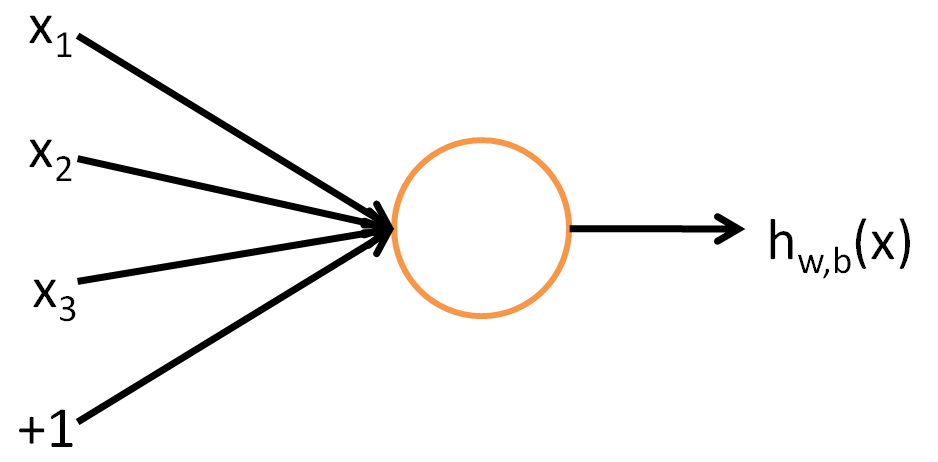
\includegraphics[width=8cm]{resource/SingleNeuron.png}
\caption{网络神经元}
\caption*{\small 来源: \url{http://ufldl.stanford.edu/tutorial/supervised/MultiLayerNeuralNetworks/}}
\label{fig:sn}
\end{figure}

将多个神经元连接为神经网络模型,如图\ref{fig:n331}
\begin{figure}[htbp]
\centering
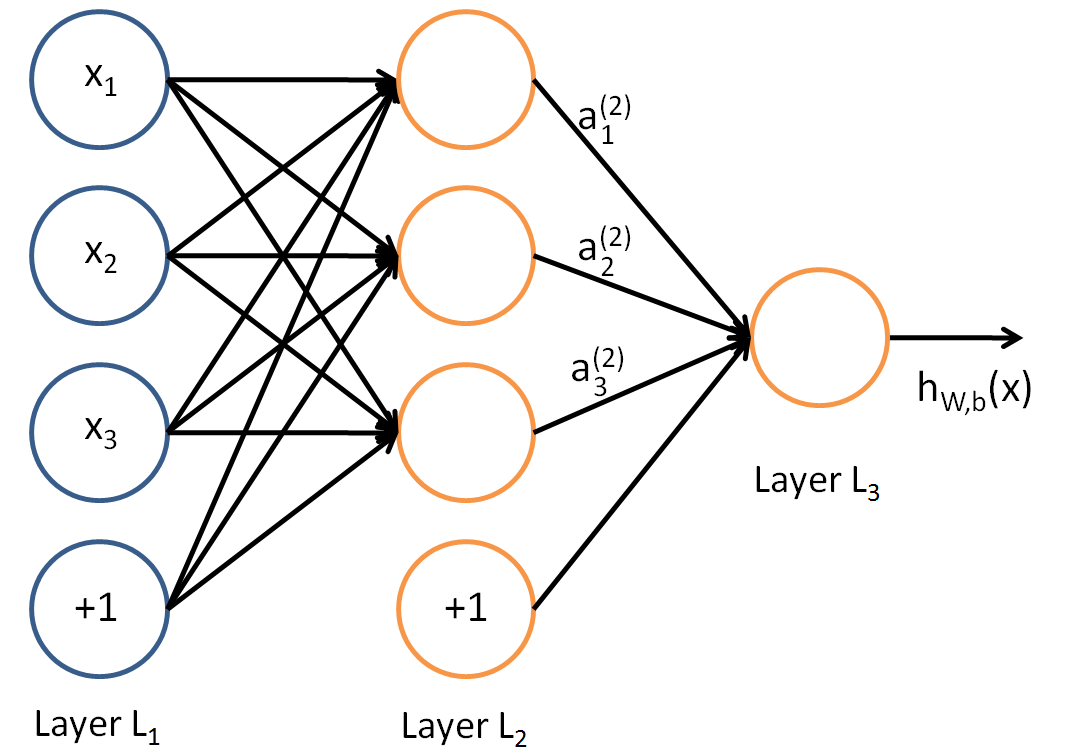
\includegraphics[width=8cm]{resource/Network331.png}
\caption{单层神经网络}
\caption*{\small 来源: \url{http://ufldl.stanford.edu/tutorial/supervised/MultiLayerNeuralNetworks/}}
\label{fig:n331}
\end{figure}

网络前向传播公式为:
\begin{align}
a_1^{(2)} &= f(W_{11}^{(1)}x_1 + W_{12}^{(1)} x_2 + W_{13}^{(1)} x_3 + b_1^{(1)})  \\
a_2^{(2)} &= f(W_{21}^{(1)}x_1 + W_{22}^{(1)} x_2 + W_{23}^{(1)} x_3 + b_2^{(1)})  \\
a_3^{(2)} &= f(W_{31}^{(1)}x_1 + W_{32}^{(1)} x_2 + W_{33}^{(1)} x_3 + b_3^{(1)})  \\
h_{W,b}(x) &= a_1^{(3)} =  f(W_{11}^{(2)}a_1^{(2)} + W_{12}^{(2)} a_2^{(2)} + W_{13}^{(2)} a_3^{(2)} + b_1^{(2)})
\end{align}

写成矩阵形式:
\begin{align}
z^{(l+1)} &= W^{(l)} a^{(l)} + b^{(l)}   \\
a^{(l+1)} &= f(z^{(l+1)})
\end{align}

多个这样的层即可连接成多层神经网络,如图\ref{fig:n3322}。网络输出层与期望输出之间可以建立损失函数,并使用梯度下降法使输出逼近期望的输出。常用的$L_2$损失函数为
\begin{align}
J(W,b; x,y) = \frac{1}{2} \left\| h_{W,b}(x) - y \right\|^2.
\end{align}

\begin{figure}[htbp]
\centering
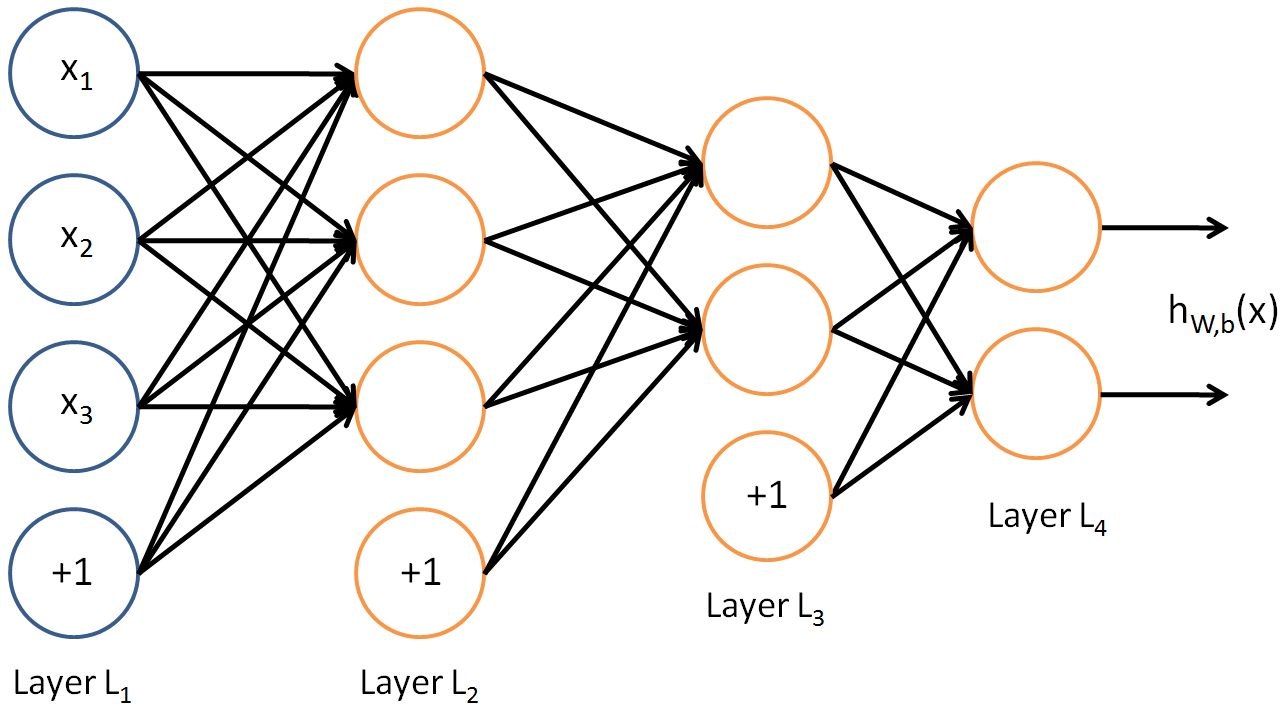
\includegraphics[width=8cm]{resource/Network3322.png}
\caption{多层神经网络}
\caption*{\small 来源: \url{http://ufldl.stanford.edu/tutorial/supervised/MultiLayerNeuralNetworks/}}
\label{fig:n3322}
\end{figure}

\section{实验结果}
错误率汇总如表\ref{tab:error}。

\begin{table}[htbp]
	\centering
	\begin{tabular}{c|c|cccc}
	\hline
	训练样本数 & 特征数 & Bayes & FLD & Linear SVM & MLP (hidden nodes=12) \\
	\hline
	\multirow{2}*{10+10} & 10 & 12.538226\% & 26.299694\% & 24.464832\% & 72.47706422\% (epoch=100)\\
		\cline{2-6}
		& 2 & 22.324159\% & 15.596330\% & 17.125382\% & 82.87461774\% (epoch=100) \\
	\hline
	\multirow{2}*{469+485} & 10 & 16.819572\% & 10.091743\% & 11.926606\% & 11.62079511\% (epoch=500) \\
		\cline{2-6}
		& 2 & 	14.067278\% & 11.620795\% & 12.232416\% & 7.339449541\% (epoch=500) \\
	\hline
	\end{tabular}
	\caption{各种方法错误率汇总}
	\label{tab:error}
\end{table}

使用两个特征和所有训练数据,得到的决策边界如图\ref{fig:db}。
\begin{figure}[htbp]
\centering
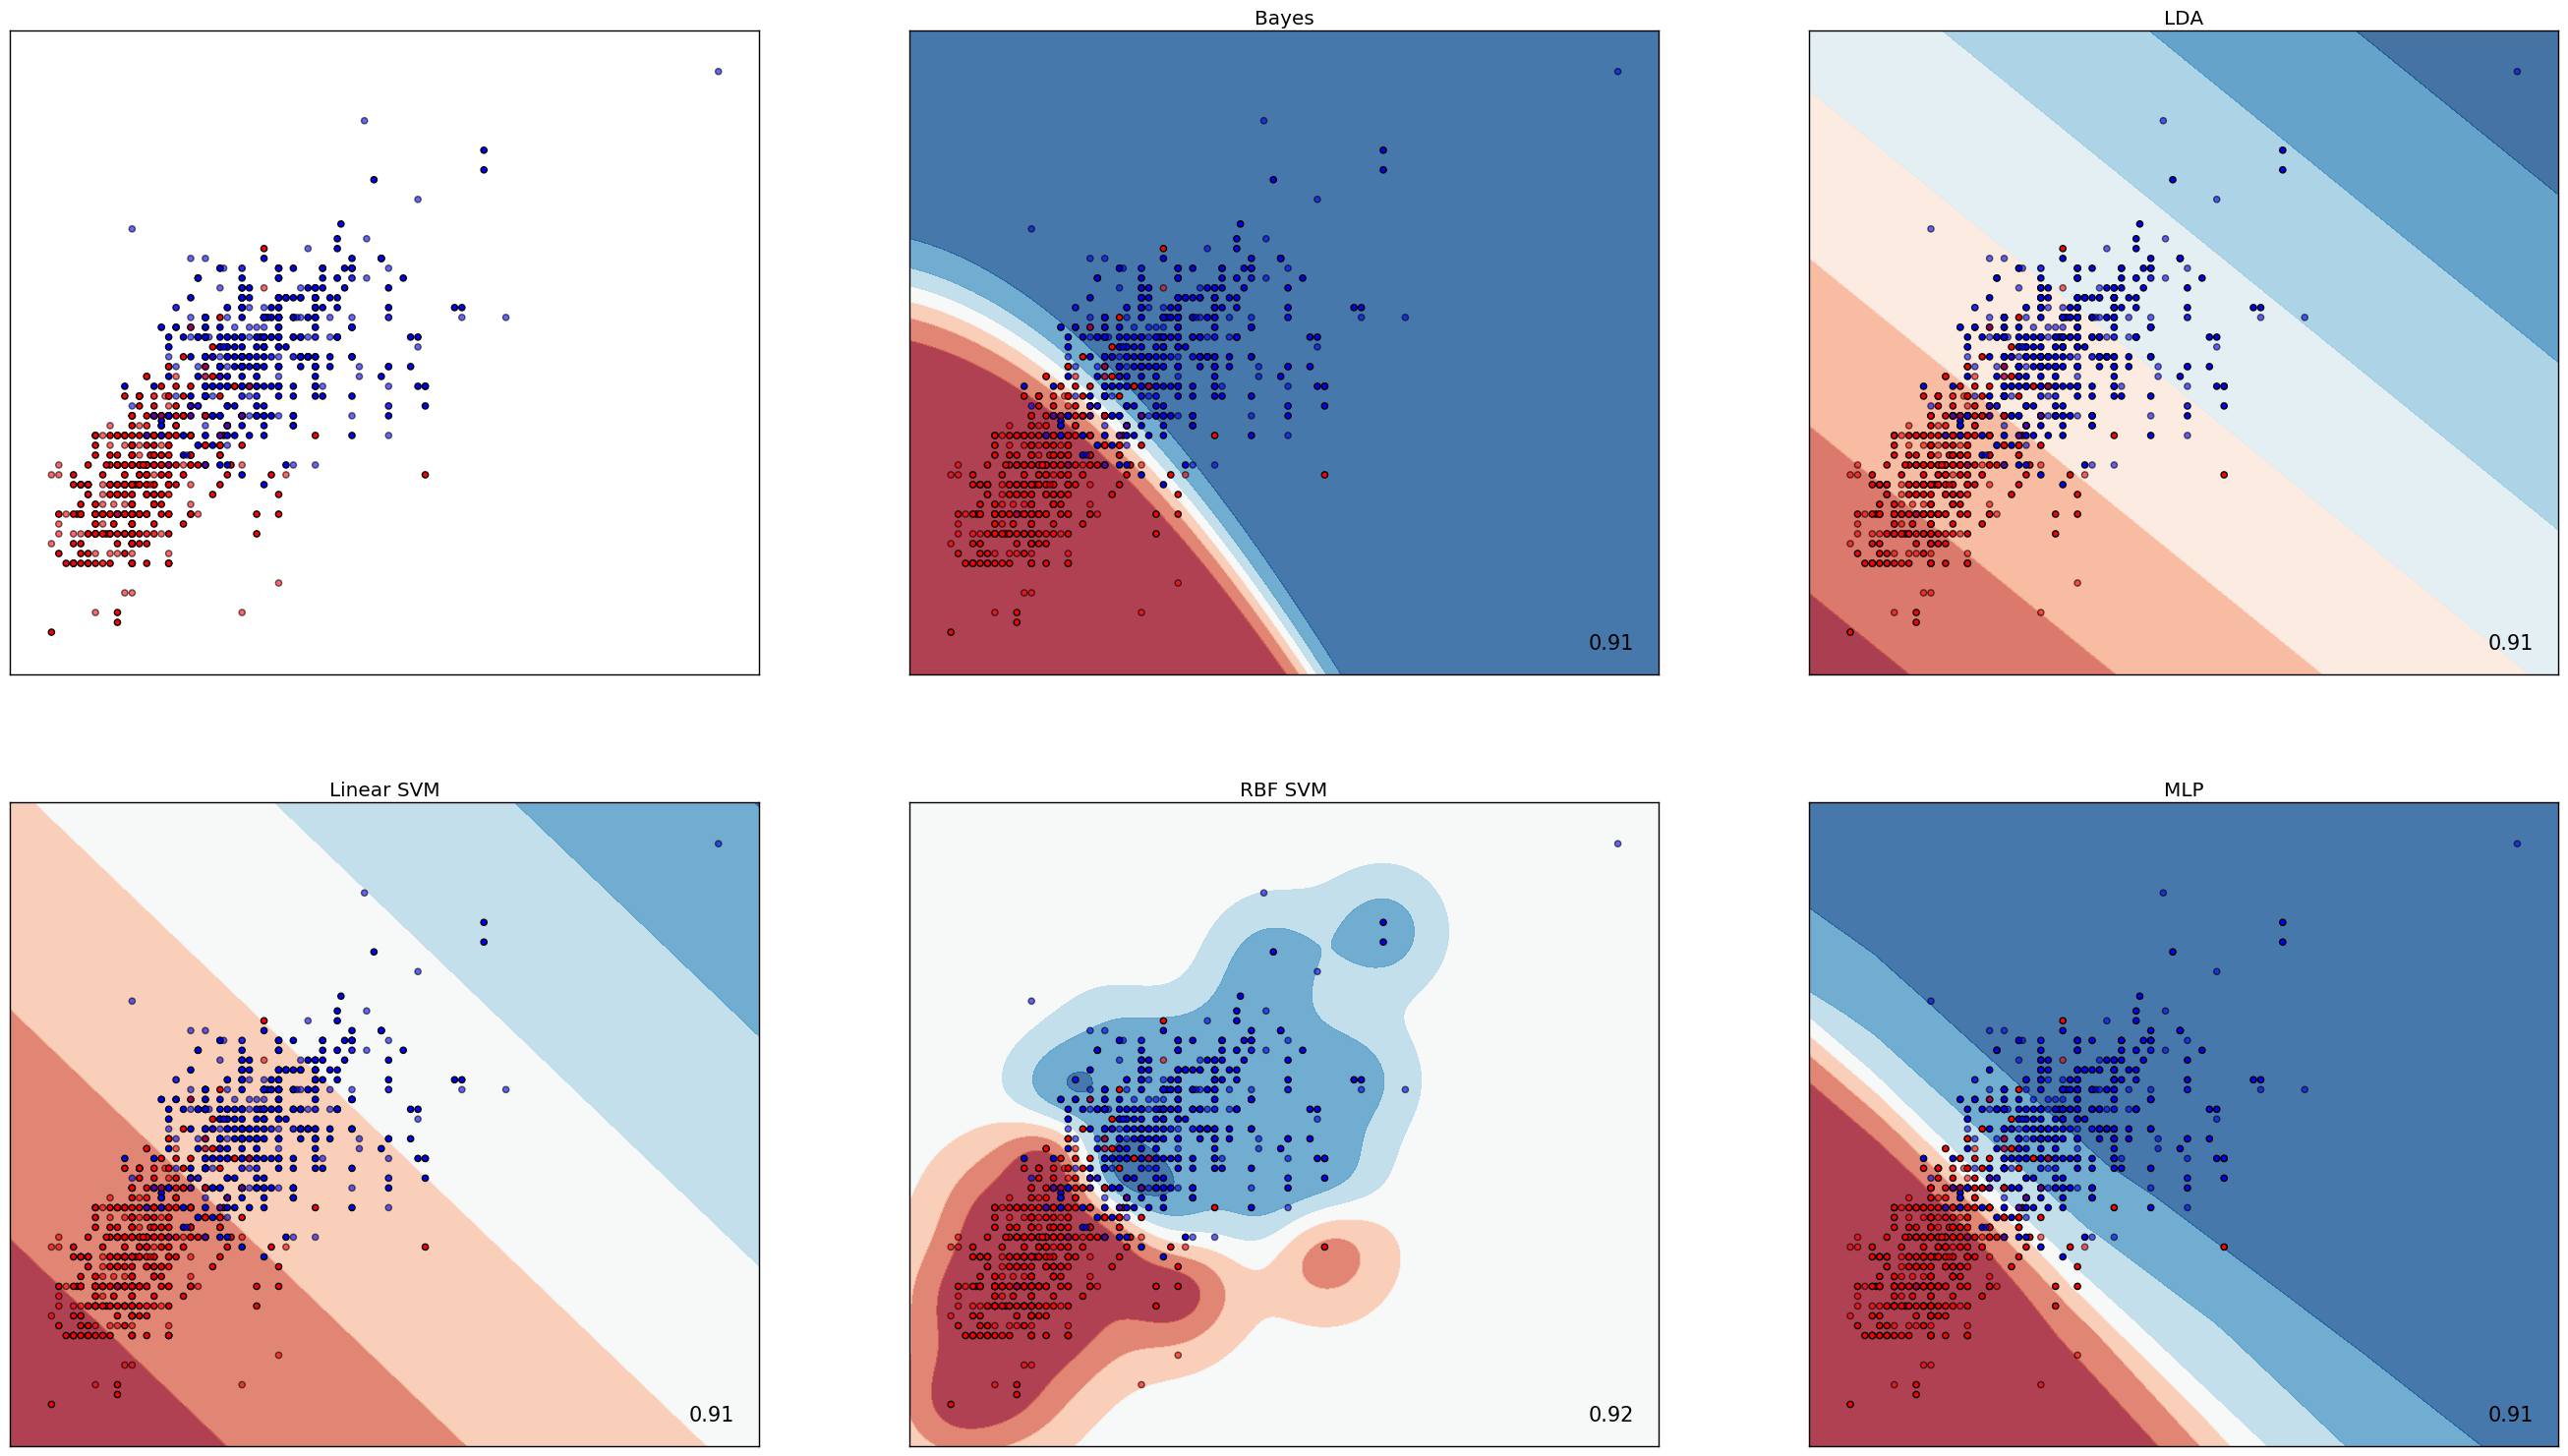
\includegraphics[width=15cm]{resource/db.png}
\caption{决策边界}
\label{fig:db}
\end{figure}

\section{分析与体会}
\subsection{训练样本数对实验结果的影响}
从实验结果来看,大部分情况下减少训练样本错误率都会上升。只有在10特征的贝叶斯最小错误率实验中出现了相反的结果。而对于神经网络来说,样本较少的情况下无法学习到可用的分类器。这说明贝叶斯最小错误率分类器在样本较少时比较有效,而神经网络在样本较多时表现很好。
\subsection{特征数对实验结果的影响}
从实验结果来看,大部分情况下使用两个特征能够取得与10个特征相近,甚至更好的结果。这可能是由于除了这两个特征外,其他特征与男、女的相关性不大,导致分类器被误导。由图\ref{fig:fr}可以看出,线性可分性较好的特征有$V1$,$V3$,$V5$,而$V6-V10$几乎无法将男女分开。程序中对此进行了追加实验,使用6-10号特征,用MLP方法进行分类,其他参数和训练的次数都相同的情况下,分类错误率高达$23.55\%$。而使用1,3,5号特征的两个或三个,达到的分类效果在MLP分类器下都很接近。
\subsection{分类方法对实验结果的影响}
这里取使用所有训练样本,两个特征的实验结果比较各种方法。可以看出,贝叶斯最小错误率分类器表现最差。原因可能是训练样本和测试样本的两类比例有很大差别,而贝叶斯方法分类时对这种比例是敏感的,先验概率均为$0.5$的假设与测试集有很大偏差。Fisher线性分类器和线性SVM效果比较接近。其中Fisher线性分类器试图取得较大的类间距离和较小的类内距离,线性SVM基于支持向量取得支持向量之间的最大距离,二者在原理上有相似之处。而线性SVM不依赖两类的比例,因此比Fisher分类器稍好。MLP方法表现最好,因为它是非线性分类。观察图\ref{fig:fr}中的$V3$、$V5$组合,显然非线性分界面更为合适。但正是由于该方法是非线性的,在训练集很小时完全学不到可用的分类器。经过对预测结果的分析,MLP在仅有20个训练样本时,对测试集的性别预测也基本是男、女各一半。而测试集实际的男、女比例约为$4:1$,故错误率在$80\%$左右,和随机预测的错误率是吻合的。

\begin{figure}
\centering
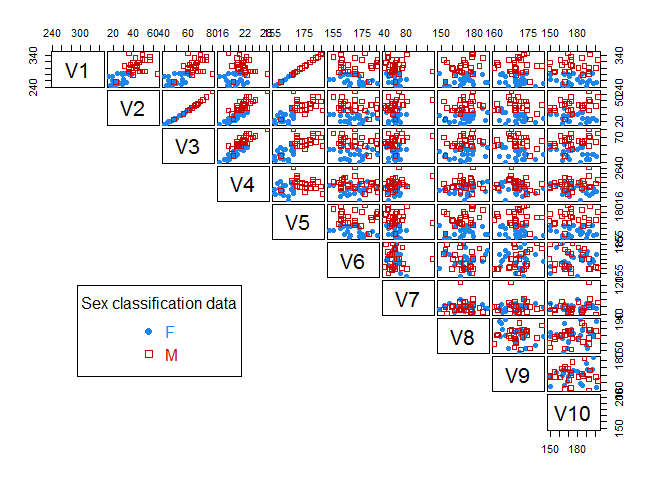
\includegraphics[width=15cm]{resource/feature_relation.png}
\caption{以任意两个特征为横纵坐标的训练数据分布图}
\label{fig:fr}
\end{figure}

\section{数据与程序说明}
\subsection{随机采样方法}
采用{\ttfamily sample}函数生成一定范围内不重复的随机整数。例如:
\begin{lstlisting}
	sample(1:size(df_train, 1), 10, replace = false)
\end{lstlisting}
函数具体说明参见 \url{http://statsbasejl.readthedocs.io/en/latest/sampling.html}。挑选出的样本参见源程序 \url{http://nbviewer.jupyter.org/github/chaonan99/university_homework/blob/pattern_recognition/h2/src/h2.ipynb}。

\subsection{程序说明}
程序采用{\ttfamily Julia}语言,由{\ttfamily IJulia}提供对{\ttfamily Jupyter Notebook}的支持。
\paragraph{简要方法描述} 见实验方法及结果部分。
\paragraph{程序来源} 源代码均为本人编写。用到的包参见源程序中的说明。
\paragraph{参数说明} 参见源程序中的说明。

\end{document}
